%%%%%%%%%%%%%%%%%%%%%%%%%%%%%%%%%%%%%%%%%%%%%%%%%%%%%%%%%%%%%%%%%%%%%
%
% VC36O Writeup Template
%
% This is a LaTeX document. LaTeX is a markup language for producing 
% documents. Your task is to fill out this
% document, then to compile this into a PDF document. 
% You will then upload this PDF to `Moodle'.
%
% 
% TO COMPILE:
% > pdflatex thisfile.tex
%
% For references to appear correctly instead of as '??', you must run 
% pdflatex twice.
%
% If you do not have LaTeX and need a LaTeX distribution:
% - Personal laptops (all common OS): www.latex-project.org/get/
%
% If you need help with LaTeX, please come to office hours. 
% Or, there is plenty of help online:
% https://en.wikibooks.org/wiki/LaTeX
%
% Good luck!
%
%%%%%%%%%%%%%%%%%%%%%%%%%%%%%%%%%%%%%%%%%%%%%%%%%%%%%%%%%%%%%%%%%%%%%%%%%%%%%%%%%%%%%%%%%%%%%%%%
%
% How to include two graphics on the same line:
% 
% \includegraphics[width=0.49\linewidth]{yourgraphic1.png}
% \includegraphics[width=0.49\linewidth]{yourgraphic2.png}
%
% How to include equations:
%
% \begin{equation}
% y = mx+c
% \end{equation}
% 
%%%%%%%%%%%%%%%%%%%%%%%%%%%%%%%%%%%%%%%%%%%%%%%%%%%%%%%%%%%%%%%%%%%%%%%%%%%%%%%%%%%%%%%%%%%%%%%%

\documentclass[11pt]{article}

\usepackage[english]{babel}
\usepackage[utf8]{inputenc}
\usepackage[colorlinks = true,
            linkcolor = blue,
            urlcolor  = blue]{hyperref}
\usepackage[a4paper,margin=1.5in]{geometry}
\usepackage{stackengine,graphicx}
\usepackage{fancyhdr}
\setlength{\headheight}{15pt}
\usepackage{microtype}
\usepackage{times}

\usepackage{float}

% Poder utilizar as matrizes
\usepackage{amsmath}

% From https://ctan.org/pkg/matlab-prettifier
\usepackage[numbered,framed]{matlab-prettifier}

\frenchspacing
\setlength{\parindent}{0cm} % Default is 15pt.
\setlength{\parskip}{0.3cm plus1mm minus1mm}

\pagestyle{fancy}
\fancyhf{}
\lhead{Project 1 Questions}
\rhead{VC36O 2018/1}
\rfoot{\thepage}

\date{}

\title{\vspace{-1cm}Project 1 Questions}


\begin{document}
\maketitle
\vspace{-3cm}
\thispagestyle{fancy}

%\section*{Instructions}
%\begin{itemize}
%  \item 4 questions.
%  \item Write code where appropriate.
%  \item Feel free to include images or equations.%
%  \item Please make this document anonymous.
%  \item \textbf{Please use only the space provided and keep the page breaks.} Please do not make new pages, nor remove pages. The document is a template to help grading.
%  \item If you really need extra space, please use new pages at the end of the document and refer us to it in your answers.
%\end{itemize}

\section*{Questions}

\paragraph{Q1:} Explicitly describe image convolution: the input, the transformation, and the output. Why is it useful for computer vision?

%%%%%%%%%%%%%%%%%%%%%%%%%%%%%%%%%%%
\paragraph{A1:} A convolução de uma imagem envolve três matrizes bidimensionais, que são: a imagem de entrada, aonde será aplicado a máscara, a máscara, que será aplicada na imagem de entrada e a imagem de saída, que será o resultado da máscara aplicado na imagem de entrada. Os passos para realizar a convolução em uma imagem são:
\begin{itemize}
	\item Fazer a borda de zeros na imagem de entrada (para um filtro de dimensões de m linhas e n colunas, preenchemos com zeros a imagem com um mínimo de m-1 linhas acima e abaixo e n-1 colunas à esquerda e à direita), como pode ser visto no exemplo abaixo.
\end{itemize}

\begin{figure}[!htb]
	\centering
	$ f = $
	$
	\begin{bmatrix}
	    0 & 0 & 0 & 0 & 0 \\
	    0 & 0 & 0 & 0 & 0 \\
	    0 & 0 & 1 & 0 & 0 \\
	    0 & 0 & 0 & 0 & 0 \\
	    0 & 0 & 0 & 0 & 0
	\end{bmatrix}
	$
	\caption{exemplo de imagem de entrada.}
	\label{fig:input_matrix}
\end{figure}

\begin{figure}[!htb]
	\centering
	$ w = $
	$
	\begin{bmatrix}
	    1 & 2 & 3 \\
	    4 & 5 & 6 \\
	    7 & 8 & 9 \\
	\end{bmatrix}
	$ % Corrigir o erro da bmatrix
	\caption{exemplo de máscara que será aplicada na imagem de entrada.}
	\label{fig:mask_correlation}
\end{figure}

\begin{figure}[!htb]
	\centering
	$ f = $
	$
	\begin{bmatrix}
	    0 & 0 & 0 & 0 & 0 & 0 & 0 & 0 & 0 \\
	    0 & 0 & 0 & 0 & 0 & 0 & 0 & 0 & 0 \\
	    0 & 0 & 0 & 0 & 0 & 0 & 0 & 0 & 0 \\
	    0 & 0 & 0 & 0 & 0 & 0 & 0 & 0 & 0 \\
	    0 & 0 & 0 & 0 & 1 & 0 & 0 & 0 & 0 \\
	    0 & 0 & 0 & 0 & 0 & 0 & 0 & 0 & 0 \\
	    0 & 0 & 0 & 0 & 0 & 0 & 0 & 0 & 0 \\
	    0 & 0 & 0 & 0 & 0 & 0 & 0 & 0 & 0 \\
	    0 & 0 & 0 & 0 & 0 & 0 & 0 & 0 & 0
	\end{bmatrix}
	$
	\caption{exemplo da imagem de entrada com a borda.}
\end{figure}

\begin{figure}[!htb]
	\begin{itemize}
		\item Antes de utilizar a máscara na convolução a mesma deve ser rotacionado em 180º.
	\end{itemize}
\end{figure}

\begin{figure}[!htb]
	\centering
	$ w = $
	$
	\begin{bmatrix}
	    9 & 8 & 7 \\
	    6 & 5 & 4 \\
	    3 & 2 & 1 \\
	\end{bmatrix}
	$ % Corrigir o erro da bmatrix
	\caption{máscara rotacionada em 180º.}
	\label{fig:mask_convolution}
\end{figure}

\begin{figure}[!htb]
	\begin{itemize}
		\item Agora aplicamos na imagem de entrada a máscara, pela fórmula abaixo.
	\end{itemize}
\end{figure}

\begin{figure}[!htb]
	\begin{equation}
		w(x, y) f(x, y) = \sum_{s = -a} ^ {a} \sum_{t = -b} ^ {b} w(s, t) f(x - s, y - t)
	\end{equation}
	\caption{fórmula da convolução.}
\end{figure}

\pagebreak
\begin{figure}[H]
	\begin{itemize}
		\item Após aplicar a fórmula acima devemos obter o seguinte resultado.
	\end{itemize}
\end{figure}

\begin{figure}[H]
	\centering
	$ w(x, y) f(x, y) = $
	$
	\begin{bmatrix}
	    0 & 0 & 0 & 0 & 0 & 0 & 0 & 0 & 0 \\
	    0 & 0 & 0 & 0 & 0 & 0 & 0 & 0 & 0 \\
	    0 & 0 & 0 & 0 & 0 & 0 & 0 & 0 & 0 \\
	    0 & 0 & 0 & 1 & 2 & 3 & 0 & 0 & 0 \\
	    0 & 0 & 0 & 4 & 5 & 6 & 0 & 0 & 0 \\
	    0 & 0 & 0 & 7 & 8 & 9 & 0 & 0 & 0 \\
	    0 & 0 & 0 & 0 & 0 & 0 & 0 & 0 & 0 \\
	    0 & 0 & 0 & 0 & 0 & 0 & 0 & 0 & 0 \\
	    0 & 0 & 0 & 0 & 0 & 0 & 0 & 0 & 0
	\end{bmatrix}
	$
	\caption{imagem de entrada após a aplicação da máscara.}
\end{figure}

\begin{figure}[!htb]
	\begin{itemize}
		\item Por fim, devemos remover a borda de zeros que adicionamos no primeiro passo.
	\end{itemize}
\end{figure}

\begin{figure}[!htb]
	\centering
	$ w(x, y) f(x, y) = $
	$
	\begin{bmatrix}
	    0 & 0 & 0 & 0 & 0 \\
	    0 & 1 & 2 & 3 & 0 \\
	    0 & 4 & 5 & 6 & 0 \\
	    0 & 7 & 8 & 9 & 0 \\
	    0 & 0 & 0 & 0 & 0 \\
	\end{bmatrix}
	$
	\caption{imagem de entrada após a aplicação da máscara e sem a borda de zeros.}
\end{figure}

Uma das importâncias da convolução na visão computacional, é que ela nos permite, por exemplo: criar imagens híbridas. Para criar esse tipo de imagem, é necessário duas imagens de entradas, sendo que uma delas nos interessa somente as baixas frequências e a outra somente as altas frequências. Para obter essas duas imagens, podemos utilizar a transformada rápida de Fourier em que a mesma emprega a convolução, que é o processo de mover uma máscara pela imagem e calcular a soma dos produtos em cada posição, como foi explicado anteriormente.

%%%%%%%%%%%%%%%%%%%%%%%%%%%%%%%%%%%

% Please leave the pagebreak
\pagebreak
\paragraph{Q2:} What is the difference between convolution and correlation? Construct a scenario which produces a different output between both operations.

\emph{Please use \href{https://www.mathworks.com/help/images/ref/imfilter.html}{$imfilter$} to experiment! Look at the `options' parameter in MATLAB Help to learn how to switch the underlying operation from correlation to convolution.}

%%%%%%%%%%%%%%%%%%%%%%%%%%%%%%%%%%%
\paragraph{A2:} A principal diferença entre a correlação e a convolução, é a máscara que se utiliza nos processos. A máscara que se utiliza na correlação está na figura \ref{fig:mask_correlation}, e a máscara que da convolução na figura \ref{fig:mask_convolution}, que basicamente é a máscara da correlação rotacionada em 180º. O processo de aplicar a máscara na imagem de entrada é o mesmo, em que movemos a máscara pela imagem e calcuamos a soma dos produtos em cada posição. Um cenário que podemos ver a diferença de saída entre essas duas operações é aplicando as máscaras que estão na figura \ref{fig:mask_correlation} e \ref{fig:mask_convolution} na matriz bidimensional de uma imagem de entrada, que está na figura \ref{fig:input_matrix}. O resultado que podemos ver da correlação e da convolução, pode ser visto respectivamente abaixo.

\begin{figure}[!htb]
	\centering
	$ w(x, y) f(x, y) = $
	$
	\begin{bmatrix}
	    0 & 0 & 0 & 0 & 0 \\
	    0 & 9 & 8 & 7 & 0 \\
	    0 & 6 & 5 & 4 & 0 \\
	    0 & 3 & 2 & 1 & 0 \\
	    0 & 0 & 0 & 0 & 0 \\
	\end{bmatrix}
	$
	\caption{resultado da correlação, após a aplicação da máscara na imagem de entrada.}
\end{figure}

\begin{figure}[!htb]
	\centering
	$ w(x, y) f(x, y) = $
	$
	\begin{bmatrix}
	    0 & 0 & 0 & 0 & 0 \\
	    0 & 1 & 2 & 3 & 0 \\
	    0 & 4 & 5 & 6 & 0 \\
	    0 & 7 & 8 & 9 & 0 \\
	    0 & 0 & 0 & 0 & 0 \\
	\end{bmatrix}
	$
	\caption{resultado da convolução, após a aplicação da máscara na imagem de entrada.}
\end{figure}

Com relação a função imfilter presente no MATLAB, se você passar para essa função apenas como parâmetro a imagem de entrada e o filtro, ele irá realizar a opção definida por padrão que no caso é a correlação, que pode ser visto na primeira linha do código abaixo. Caso você deseje realizar a operação de convolução, além de passar a matriz bidimensional da imagem de entrada e o filtro, você deve passar um terceiro parâmetro que no caso é ``conv", que se refere a operação de convolução. Essa invocação de função pode ser visto na segunda linha do código abaixo.

\begin{lstlisting}[style=Matlab-editor]
imfilter(entrada, filtro)
imfilter(entrada, filtro, 'conv')
\end{lstlisting}

%%%%%%%%%%%%%%%%%%%%%%%%%%%%%%%%%%%

% Please leave the pagebreak
\pagebreak
\paragraph{Q3:} What is the difference between a high pass filter and a low pass filter in how they are constructed, and what they do to the image? Please provide example kernels and output images.

%%%%%%%%%%%%%%%%%%%%%%%%%%%%%%%%%%%
%Ref: http://www.ufrgs.br/engcart/PDASR/vizin.html
\paragraph{A3:} A diferença entre um filtro passa-alta de um filtro passa-baixa, é que o filtro passa-alta aceita altas frequências, e tem como papel realçar as pequenas diferenças locais, associadas às frequências espaciais altas. O filtro passa-baixa é um filtro que aceita baixas frequências, e produz na imagem quando aplicado um efeito de borramento, de suavizar a imagem. O filtro passa-baixa pode ser montado de três maneiras, podendo ser um filtro passa-baixa ideias, passa-baixa Butterworth e passa-baixa gaussianos. Para montar o passa-baixa ideais, deve ser utilizar a seguinte função:

\[
	H(u, v) = 
	\begin{cases} 
        1 & \text{if $D(u, v) \leq D_0$}\\
        0 & \text{if $D(u, v) > D_0$}\\
   \end{cases}
\]

onde $D_0$ é uma constante positiva, e $D(u, v)$ é a distância entre um ponto (u, v) no domínio da frequência e o centro do retângulo de frequência. Já $D(u, v)$ é obtido através da seguinte fórmula:

\begin{equation}
	D(u, v) = \sqrt{(u - P / 2)^2 + (v - Q / 2)^2}
\end{equation}

onde $P$ e $Q$ são dados pelas respectivas fórmulas:

\begin{equation}
	P \geq 2 * M - 1
\end{equation}

\begin{equation}
	Q \geq 2 * N - 1
\end{equation}

onde $M$ e $N$ são altura e largura da imagem onde será aplicado o filtro, respectivamente. Uma outra maneira de construir um filtro passa-baixa, é você construir um filtro passa-baixa Butterworth pela seguinte fórmula:

\begin{equation}
	H(u , v) = 1 / 1 + [D(u, v) / D_0]^{2n}
\end{equation}

onde $n$ é a ordem do filtro. Por fim, a última maneira de se construir um filtro passa-baixa é o mesmo sendo um filtro passa-baixa gaussiano que pode se utilizar a seguinte fórmula:

\begin{equation}
	H(u , v) = e ^ {-D^2(u, v) / 2 D_0^2}
\end{equation}

onde $e$ é o número de Euler. Já para o filtro passa-alta também tem três opções que são: filtro passa alta-ideiais, o Butterworth e o gaussianos, em que a fórmula para suas construções podem ser vistar abaixo, respectivamente:

\[
	H(u, v) = 
	\begin{cases} 
        0 & \text{if $D(u, v) \leq D_0$}\\
        1 & \text{if $D(u, v) > D_0$}\\
   \end{cases}
\]

\begin{equation}
	H(u , v) = 1 / 1 + [D_0 / D(u, v)]^{2n}
\end{equation}

\begin{equation}
	H(u , v) = 1 - e ^ {-D^2(u, v) / 2 D_0^2}
\end{equation}

Abaixo iremos mostrar uma imagem na qual aplicaremos um filtro passa-baixa gaussiano, uma parte do filtro passa-baixa gaussiano e o resultado obtido, respectivamente.

\begin{figure}[!htb]
  \centering
  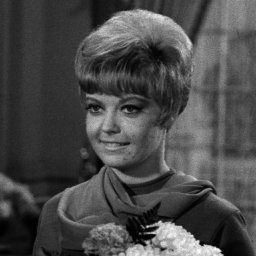
\includegraphics[scale=0.5]{pratica6.png}
  \caption{imagem de entrada aonde será aplicado o filtro passa-baixa gaussiano.}
  %\label{fig:local-np=4}
\end{figure}

\begin{figure}[!htb]
	\centering
	$
	\begin{bmatrix}
	    7.0015e-72  & 1.3262e-71 & 2.5056e-71 & 4.7223e-71 & \dots \\
	    1.3262e-71  & 2.5119e-71 & 4.7459e-71 & 8.9445e-71 & \dots \\
   		2.5056e-71  & 4.7459e-71 & 8.9669e-71 & 1.6900e-70 & \dots \\
   		4.7223e-71  & 8.9445e-71 & 1.6900e-70 & 3.1850e-70 & \dots \\
   		8.8777e-71  & 1.6815e-70 & 3.1771e-70 & 5.9877e-70 & \dots \\
   		1.6648e-70  & 3.1533e-70 & 5.9578e-70 & 1.1229e-69 & \dots \\
   		3.1142e-70  & 5.8985e-70 & 1.1145e-69 & 2.1004e-69 & \dots \\
   		5.8107e-70  & 1.1006e-69 & 2.0795e-69 & 3.9191e-69 & \dots \\
   		1.0815e-69  & 2.0485e-69 & 3.8705e-69 & 7.2945e-69 & \dots \\
   		2.0080e-69  & 3.8033e-69 & 7.1859e-69 & 1.3543e-68 & \dots \\
   		\vdots & \vdots & \vdots & \vdots & \ddots\\
	\end{bmatrix}
	$
	\caption{parte do filtro passa-baixa gaussiano.}
\end{figure}

\begin{figure}[!htb]
  \centering
  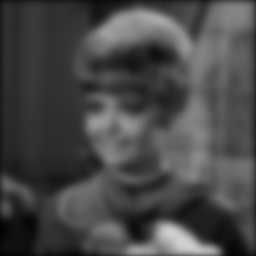
\includegraphics[scale=0.5]{final.png}
  \caption{resultado após a aplicação do filtro passa-baixa gaussiano.}
  %\label{fig:local-np=4}
\end{figure}

%%%%%%%%%%%%%%%%%%%%%%%%%%%%%%%%%%%

% Please leave the pagebreak
\pagebreak
\paragraph{Q4:} Explain the code in file \emph{$gen\textunderscore hybrid\textunderscore image\textunderscore fft.m$}. What each line is supposed to do? What does the function \emph{H()} do?


%%%%%%%%%%%%%%%%%%%%%%%%%%%%%%%%%%%
\paragraph{A4:}


Abaixo está o código do arquivo gen\textunderscore hybrid\textunderscore image\textunderscore fft.m.

\begin{lstlisting}[style=Matlab-editor]
% Cria um padding
b = padarray(image1, size(image1), "zeros", "post");

% Converte para double
c = im2double(b(:, :, 1:3));

%Faz o padding da imagem
d = fft2(c);

%Centraliza a transformada de fourier
d = fftshift(d);

% Pega as dimensoes da vaariavel c
[n m o] = size(c);

% Faz uma matriz de zeros com as dimensoes de n e m
h = zeros([n, m]);

%Construindo o filtro passa-baixa
for i = 1:n
  for j = 1:m
    h(i, j) = H(i, j, size(c), cutoff_frequency);
  end
end

% Multiplicando a matriz de transformada de Fourier pelo filtro
g = d.*h;

% Descentralizando a matriz
g = ifftshift(g);

% Aplicando a transformada inversa rapida
at = ifft2(g);

% Tira os valores negativos de at
at = abs(at);

% Pega as dimensoes da imagem 1
[x y o] = size(image1);

% Extrai da regiao X e Y
atc = at(1:x, 1:y, :);

% Atribuindo a imagem final
low_frequencies = atc;

%%%%%%%%%%%%%%%%%%%%%%
%%%% ALTA FREQUENCIA 
%%%%%%%%%%%%%%%%%%%%%%
% Cria um padding
b = padarray(image2, size(image2), "zeros", "post");

% Converte para double
c = im2double(b(:, :, 1:3));

%Faz o padding da imagem
d = fft2(c);

%Centraliza a transformada de fourier
d = fftshift(d);

% Pega as dimensoes da vaariavel c
[n m o] = size(c);

% Faz uma matriz de zeros com as dimensoes de n e m
h = zeros([n, m]);
for i = 1:n
  for j = 1:m
    h(i, j) = H(i, j, size(c), cutoff_frequency);
  end
end

% Inverter a transformada
invert = ones(size(im2uint8(h)));
h = invert .- h;

% Multiplicando a matriz de transformada de Fourier pelo filtro
g = d.*h;

% Descentralizando a matriz
g = ifftshift(g);

% Aplicando a transformada inversa rapida
at = ifft2(g);

% Pega as dimensoes da imagem 2
[x y o] = size(image2);

% Extrai da regiao X e Y
atc = at(1:x, 1:y, :);

% Atribuindo a imagem final
high_frequencies = atc;

% Combine the high frequencies and low frequencies
hybrid_image = abs(low_frequencies + high_frequencies);
\end{lstlisting}



%%%%%%%%%%%%%%%%%%%%%%%%%%%%%%%%%%%


% If you really need extra space, uncomment here and use extra pages after the last question.
% Please refer here in your original answer. Thanks!
%\pagebreak
%\paragraph{AX.X Continued:} Your answer continued here.



\end{document}